\documentclass[12pt,letterpaper]{article}

% Evidencia: GA4-220501095-AA3-EV03
% Compilar con: latexmk -pdf GA4-220501095-AA3-EV03.tex
% Guarda la imagen del diagrama con el nombre:
% diagrama_despliegue_sac.jpg
% en la misma carpeta de este archivo .tex.

\usepackage[spanish,es-nodecimaldot,shorthands=off]{babel}
\usepackage[T1]{fontenc}
\usepackage[utf8]{inputenc}
\usepackage{lmodern}
\usepackage{geometry}
\usepackage{setspace}
\usepackage{array}
\usepackage{longtable}
\usepackage{enumitem}
\usepackage{xcolor}
\usepackage{titlesec}
\usepackage{fancyhdr}
\usepackage{graphicx}
\usepackage{pdflscape}
\usepackage{float}
\usepackage{hyperref}
\usepackage{ragged2e}
\usepackage{makecell}

\newcolumntype{Y}[1]{>{\RaggedRight\arraybackslash}p{#1}}

% ==================== DATOS EDITABLES ====================
\newcommand{\institucion}{Servicio Nacional de Aprendizaje -- SENA}
\newcommand{\programa}{Analisis y Desarrollo de Software}
\newcommand{\tituloTrabajo}{Diagrama de despliegue para caso de estudio y proyecto de software}
\newcommand{\codigoEvidencia}{GA4-220501095-AA3-EV03}
\newcommand{\aprendiz}{Kevin Andres Granados Daza}
\newcommand{\instructor}{[Jesus Ramirez]}
\newcommand{\ficha}{[3389015]}
\newcommand{\ciudad}{Bogota D. C.}
\newcommand{\fechaEntrega}{[25 de septiembre de 2026]}
% ==========================================================

\geometry{top=2.54cm,bottom=2.54cm,left=2.54cm,right=2.54cm}
\onehalfspacing
\setlength{\parindent}{1.27cm}
\setlength{\parskip}{0pt}
\setlength{\headheight}{15pt}
\setlength{\LTpre}{0pt}
\setlength{\LTpost}{0pt}

\pagestyle{fancy}
\fancyhf{}
\fancyhead[L]{\codigoEvidencia}
\fancyhead[R]{\thepage}
\renewcommand{\headrulewidth}{0pt}

\titleformat{\section}{\normalfont\Large\bfseries\centering}{\thesection.}{0.5em}{}
\titleformat{\subsection}{\normalfont\large\bfseries}{\thesubsection.}{0.5em}{}

\begin{document}

% ==================== PORTADA ====================
\begin{titlepage}
    \centering
    \vspace*{2.5cm}
    {\Large \tituloTrabajo\par}
    \vfill
    {\large \aprendiz\par}
    \vspace{1.5cm}
    {\large \institucion\par}
    {\large \programa\par}
    \vspace{1cm}
    {\large Evidencia: \codigoEvidencia\par}
    \vspace{1cm}
    {\large Instructor: \instructor\par}
    {\large Ficha: \ficha\par}
    \vfill
    {\large \ciudad\par}
    {\large \fechaEntrega\par}
\end{titlepage}

% ==================== INTRODUCCION ====================
\section{Introduccion}

El diagrama de despliegue es un diagrama UML que permite representar la distribucion fisica de los componentes de software en los recursos tecnologicos donde se ejecutan. Por medio de este diagrama es posible identificar los dispositivos de los usuarios, los servidores, los entornos de ejecucion, los artefactos desplegados y las conexiones necesarias para que una aplicacion funcione.

En el presente documento se presenta el diagrama de despliegue del Sistema de Gestion de Citas para Atencion de Servicios SAC. La solucion se plantea como una aplicacion web desarrollada en PHP 8, ejecutada en un servidor web Apache y conectada a una base de datos MariaDB. El diagrama permite visualizar la relacion entre el navegador del usuario, la aplicacion web y la base de datos, teniendo en cuenta la arquitectura por capas y los requisitos definidos para el proyecto.

% ==================== OBJETIVO ====================
\section{Objetivo}

Representar mediante un diagrama de despliegue UML la arquitectura fisica del Sistema de Gestion de Citas para Atencion de Servicios SAC, identificando los nodos, artefactos, entornos de ejecucion, protocolos de comunicacion y mecanismos que permiten cumplir los requisitos funcionales y no funcionales de la solucion.

% ==================== ARQUITECTURA ====================
\section{Arquitectura de software definida}

Para el Sistema de Gestion de Citas SAC se definio una arquitectura por capas, apoyada en el patron Modelo--Vista--Controlador (MVC), una capa de servicios y el patron Repository. Esta estructura separa las responsabilidades de la aplicacion y permite mantener organizada la interaccion entre la interfaz de usuario, las reglas de negocio y el acceso a la informacion almacenada.

La capa de presentacion contiene las vistas que el usuario visualiza desde el navegador web. Los controladores reciben las solicitudes realizadas por clientes y administradores. La capa de negocio implementa reglas como la validacion de horarios, el control de estados de una cita y la restriccion de citas duplicadas. Finalmente, la capa de acceso a datos consulta y actualiza la informacion de MariaDB mediante repositorios.

La aplicacion se desarrolla en PHP 8 y se ejecuta mediante Apache HTTP Server. Durante el desarrollo puede utilizarse XAMPP como entorno local, mientras que en produccion la solucion puede alojarse en un servidor web o servicio de hosting compatible con PHP y MariaDB.

% ==================== DIAGRAMA ====================
\section{Diagrama de despliegue}

La Figura~\ref{fig:despliegue-sac} representa la disposicion fisica de los elementos principales del sistema. El usuario accede desde un computador, portatil o dispositivo movil mediante un navegador web. Las solicitudes se envian al servidor web utilizando HTTP o HTTPS. Apache y PHP 8 ejecutan la aplicacion SAC-WebApp, la cual procesa la logica del sistema y realiza consultas a la base de datos MariaDB mediante una conexion TCP/IP por el puerto 3306.


\begin{figure}[H]
    \centering
    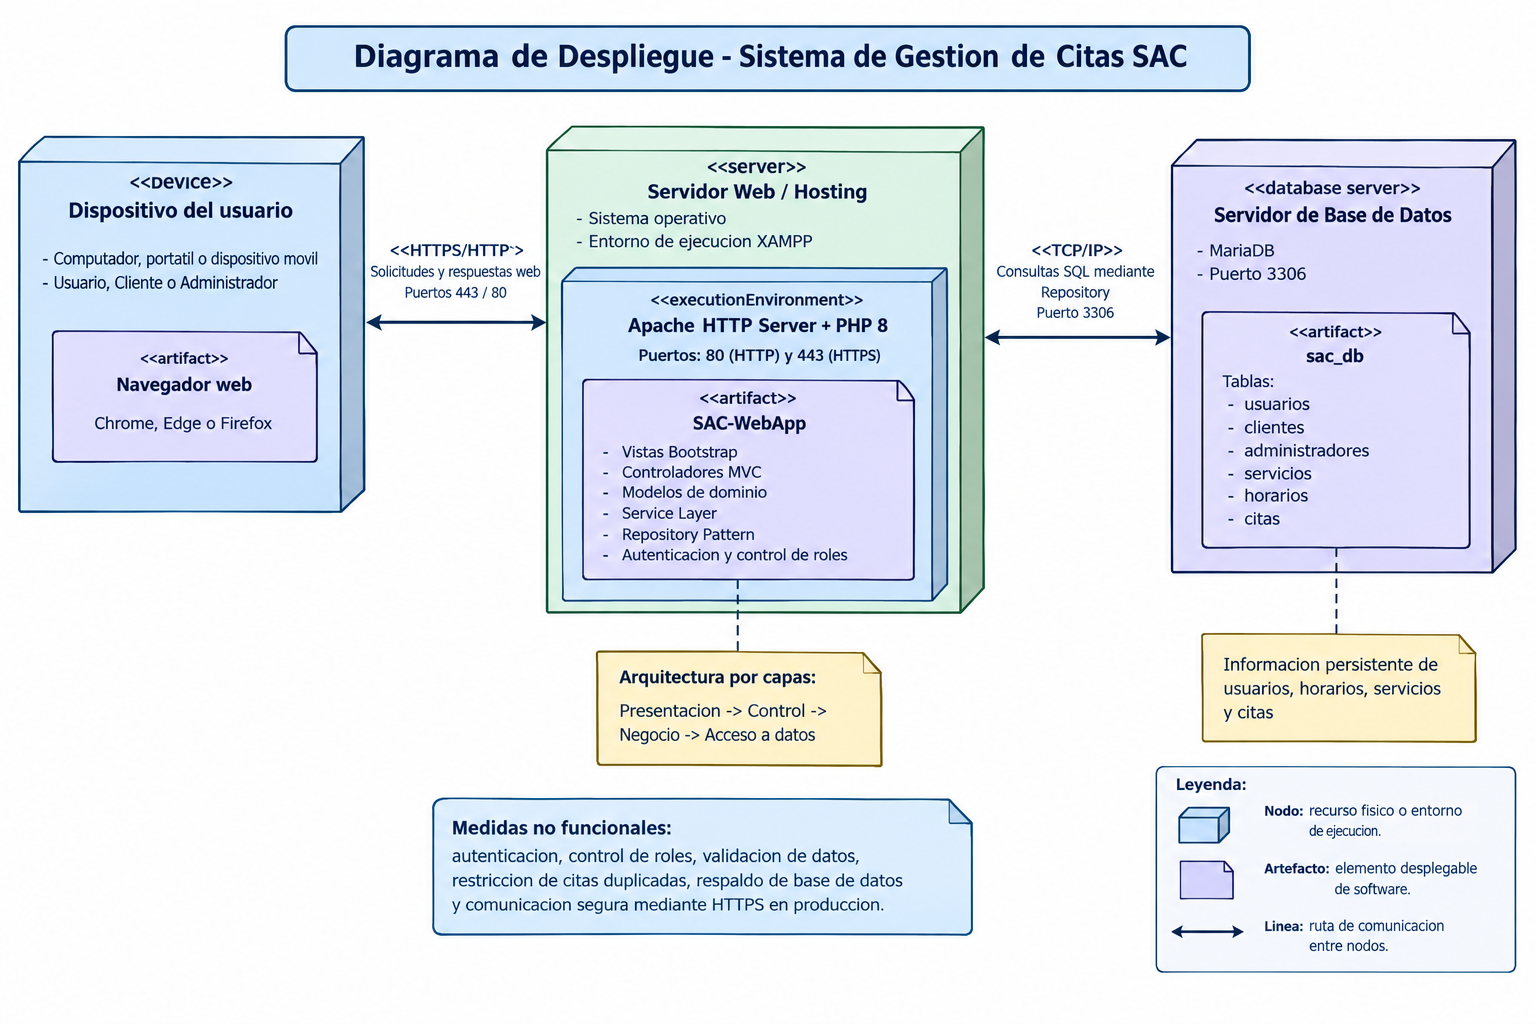
\includegraphics[width=1\textwidth]{diagrama_despliegue_sac.png}
    \caption{Diagrama de despliegue del Sistema de Gestion de Citas SAC.}
    \label{fig:despliegue-sac}
\end{figure}


% ==================== DESCRIPCION ====================
\section{Descripcion de nodos, artefactos y conexiones}

\begin{center}
\small
\setlength{\tabcolsep}{5pt}
\renewcommand{\arraystretch}{1.20}

\begin{longtable}{|Y{3.15cm}|Y{3.65cm}|Y{8cm}|}
\hline
\textbf{Elemento} & \textbf{Tipo UML} & \textbf{Descripcion} \\
\hline
\endfirsthead

\hline
\textbf{Elemento} & \textbf{Tipo UML} & \textbf{Descripcion} \\
\hline
\endhead

\hline
\endfoot

\hline
\endlastfoot

Dispositivo del usuario & \texttt{<<device>>} & Representa el computador, portatil o dispositivo movil utilizado por clientes, usuarios o administradores para acceder al sistema. \\
\hline

Navegador web & \texttt{<<artifact>>} & Es el software utilizado para visualizar la aplicacion e interactuar con sus funciones. Puede ser Chrome, Edge, Firefox u otro navegador compatible. \\
\hline

Servidor web / hosting & \texttt{<<server>>} & Nodo que aloja la aplicacion web. Incluye el sistema operativo y el entorno requerido para atender solicitudes de los usuarios. \\
\hline

Apache HTTP Server + PHP 8 & \texttt{<<executionEnvironment>>} & Entorno de ejecucion encargado de recibir peticiones web y ejecutar el codigo PHP de la aplicacion. Utiliza los puertos 80 para HTTP y 443 para HTTPS. \\
\hline

SAC-WebApp & \texttt{<<artifact>>} & Aplicacion web desplegada. Contiene vistas Bootstrap, controladores MVC, modelos de dominio, servicios, repositorios y mecanismos de autenticacion y control de roles. \\
\hline

Servidor de base de datos & \texttt{<<database server>>} & Nodo que ejecuta MariaDB y procesa las consultas necesarias para almacenar, consultar, actualizar o eliminar informacion. \\
\hline

sac\_db & \texttt{<<artifact>>} & Base de datos del sistema. Almacena la informacion de usuarios, clientes, administradores, servicios, horarios y citas. \\
\hline

HTTPS / HTTP & Ruta de comunicacion & Enlace entre el navegador y el servidor web. Permite enviar solicitudes y recibir respuestas de la aplicacion; HTTPS debe utilizarse en produccion para proteger la informacion transmitida. \\
\hline

TCP/IP -- Puerto 3306 & Ruta de comunicacion & Conexion entre SAC-WebApp y MariaDB. Permite ejecutar consultas SQL a traves de la capa de acceso a datos y los repositorios. \\
\hline
\end{longtable}
\end{center}

% ==================== REQUISITOS ====================
\section{Cumplimiento de requisitos}

El diagrama de despliegue representa la infraestructura necesaria para que el sistema cumpla con los requisitos funcionales y no funcionales definidos para el Sistema de Gestion de Citas SAC.

\begin{center}
\small
\setlength{\tabcolsep}{5pt}
\renewcommand{\arraystretch}{1.20}

\begin{longtable}{|Y{2.4cm}|Y{6.3cm}|Y{6.1cm}|}
\hline
\textbf{Tipo} & \textbf{Requisito} & \textbf{Elemento que contribuye al cumplimiento} \\
\hline
\endfirsthead
\hline
\textbf{Tipo} & \textbf{Requisito} & \textbf{Elemento que contribuye al cumplimiento} \\
\hline
\endhead
\hline
\endfoot
\hline
\endlastfoot

Funcional & Registro, autenticacion y control de acceso de usuarios. & SAC-WebApp, controladores MVC, autenticacion y control de roles. \\
\hline

Funcional & Consulta de horarios y servicios disponibles. & Vistas Bootstrap, capa de negocio, repositorios y tablas de servicios y horarios. \\
\hline

Funcional & Solicitud, confirmacion, cancelacion y reprogramacion de citas. & Controladores, servicios de negocio, validaciones y tabla de citas en sac\_db. \\
\hline

Funcional & Administracion de horarios y gestion de la informacion por parte del administrador. & Control de roles, capa de negocio, repositorios y MariaDB. \\
\hline

No funcional & Mantenibilidad y facilidad para agregar nuevas funcionalidades. & Arquitectura por capas, MVC, Service Layer y Repository Pattern. \\
\hline

No funcional & Seguridad y proteccion de la informacion. & Autenticacion, control de roles, validacion de datos y HTTPS en produccion. \\
\hline

No funcional & Integridad de la informacion y prevencion de citas duplicadas. & Reglas de negocio, validaciones y persistencia controlada en MariaDB. \\
\hline

No funcional & Disponibilidad y recuperacion de datos. & Servidor web, servidor MariaDB y respaldos periodicos de la base de datos. \\
\hline
\end{longtable}
\end{center}

% ==================== CONCLUSION ====================
\section{Conclusiones}

El diagrama de despliegue permitio representar la ubicacion fisica y la comunicacion entre los elementos principales del Sistema de Gestion de Citas SAC. Se identifico que el usuario accede desde un navegador web a una aplicacion desarrollada en PHP 8 y ejecutada mediante Apache, mientras que la informacion se almacena y consulta en una base de datos MariaDB.

La distribucion propuesta permite mantener separadas la presentacion, la logica de negocio y el acceso a datos. Esto facilita el mantenimiento de la aplicacion, la realizacion de pruebas y la incorporacion de nuevas funcionalidades. Ademas, el uso de autenticacion, control de roles, validaciones, respaldo de datos y comunicacion HTTPS contribuye al cumplimiento de requisitos no funcionales relacionados con seguridad, confiabilidad y disponibilidad.

En conclusion, el diagrama de despliegue evidencia que la arquitectura seleccionada permite ejecutar el sistema de manera organizada y escalable, manteniendo una relacion clara entre los usuarios, la aplicacion web y la base de datos.

\end{document}
